\documentclass[xcolor=dvipsnames]{beamer}
\usetheme[navigation]{UMONS}
\usepackage[utf8]{inputenc}
\usepackage{graphicx}
\usepackage{wrapfig}
\usepackage{caption}
\usepackage{hyperref}
\usepackage{url}
\usepackage{color}
\usepackage{tikz}
%\usepackage{fourier, heuristica}
\usepackage{array, booktabs}
\usepackage{graphicx}
%\usepackage[x11names]{xcolor}
\usepackage{colortbl}
\usepackage{caption}
\DeclareCaptionFont{SkyBlue}{\color{SkyBlue}}

\newcommand{\foo}{\color{SkyBlue}\makebox[0pt]{\textbullet}\hskip-0.5pt\vrule width 1pt\hspace{\labelsep}}

\renewcommand{\arraystretch}{1.9}
\newcommand{\green}[1]{\textcolor{ForestGreen}{#1}}
\newcommand{\red}[1]{\textcolor{red}{#1}}

\title{Blockchain}
\author[G.Jérémy, D.Arman, L. Semih]{Gheysen Jérémy, Davidyan Arman, Locqueneux Semih}
\date{24 Avril 2018}
\institute[]{%
 Faculté des Sciences\\
  Université de Mons
  \\[2ex]
  
\includegraphics[height=4ex]{UMONS}\hspace{2em}%
  \raisebox{-1ex}{
\includegraphics[height=6ex]{UMONS_FS}}
}

\begin{document}

\maketitle

\section{Introduction}

\begin{frame}{Introduction}{Historique}
\vspace{-0.5cm}
	\begin{table}
		\renewcommand\arraystretch{1.4}\arrayrulecolor{SkyBlue}
		\vskip -1.5ex

		\begin{tabular}{@{\,}r <{\hskip 2pt} !{\foo} >{\raggedright\arraybackslash}p{10cm}}
		
			\toprule
			\addlinespace[1.5ex]
			1991 & Premier travail sur une \textbf{chaîne sécurisée de blocs} par \textit{Haber et 	Stornetta}. \\
			1992 & Incorporation des \textbf{Merkle Trees} au design par \textit{Bayer, Haber et Stornetta}. \\
			2008 & Première conceptualisation en cryptomonnaie -- \textbf{BitCoin} par 	\textit{Satoshi Nakamoto}.\\
			2014 & Taille de la blockchain Bitcoin : 20 GB -- BitCoin : 600\$. \\
			2017 & Taille de la blockchain Bitcoin : 100 GB -- BitCoin : 1500\$. \\
			2018 & Taille de la blockchain Bitcoin : 164 GB -- BitCoin : 8000\$. \\
			
		\end{tabular}
	\end{table}
	
\end{frame}

\begin{frame}{Introduction}{Définition}
\vspace{-1cm}
	\begin{center}
		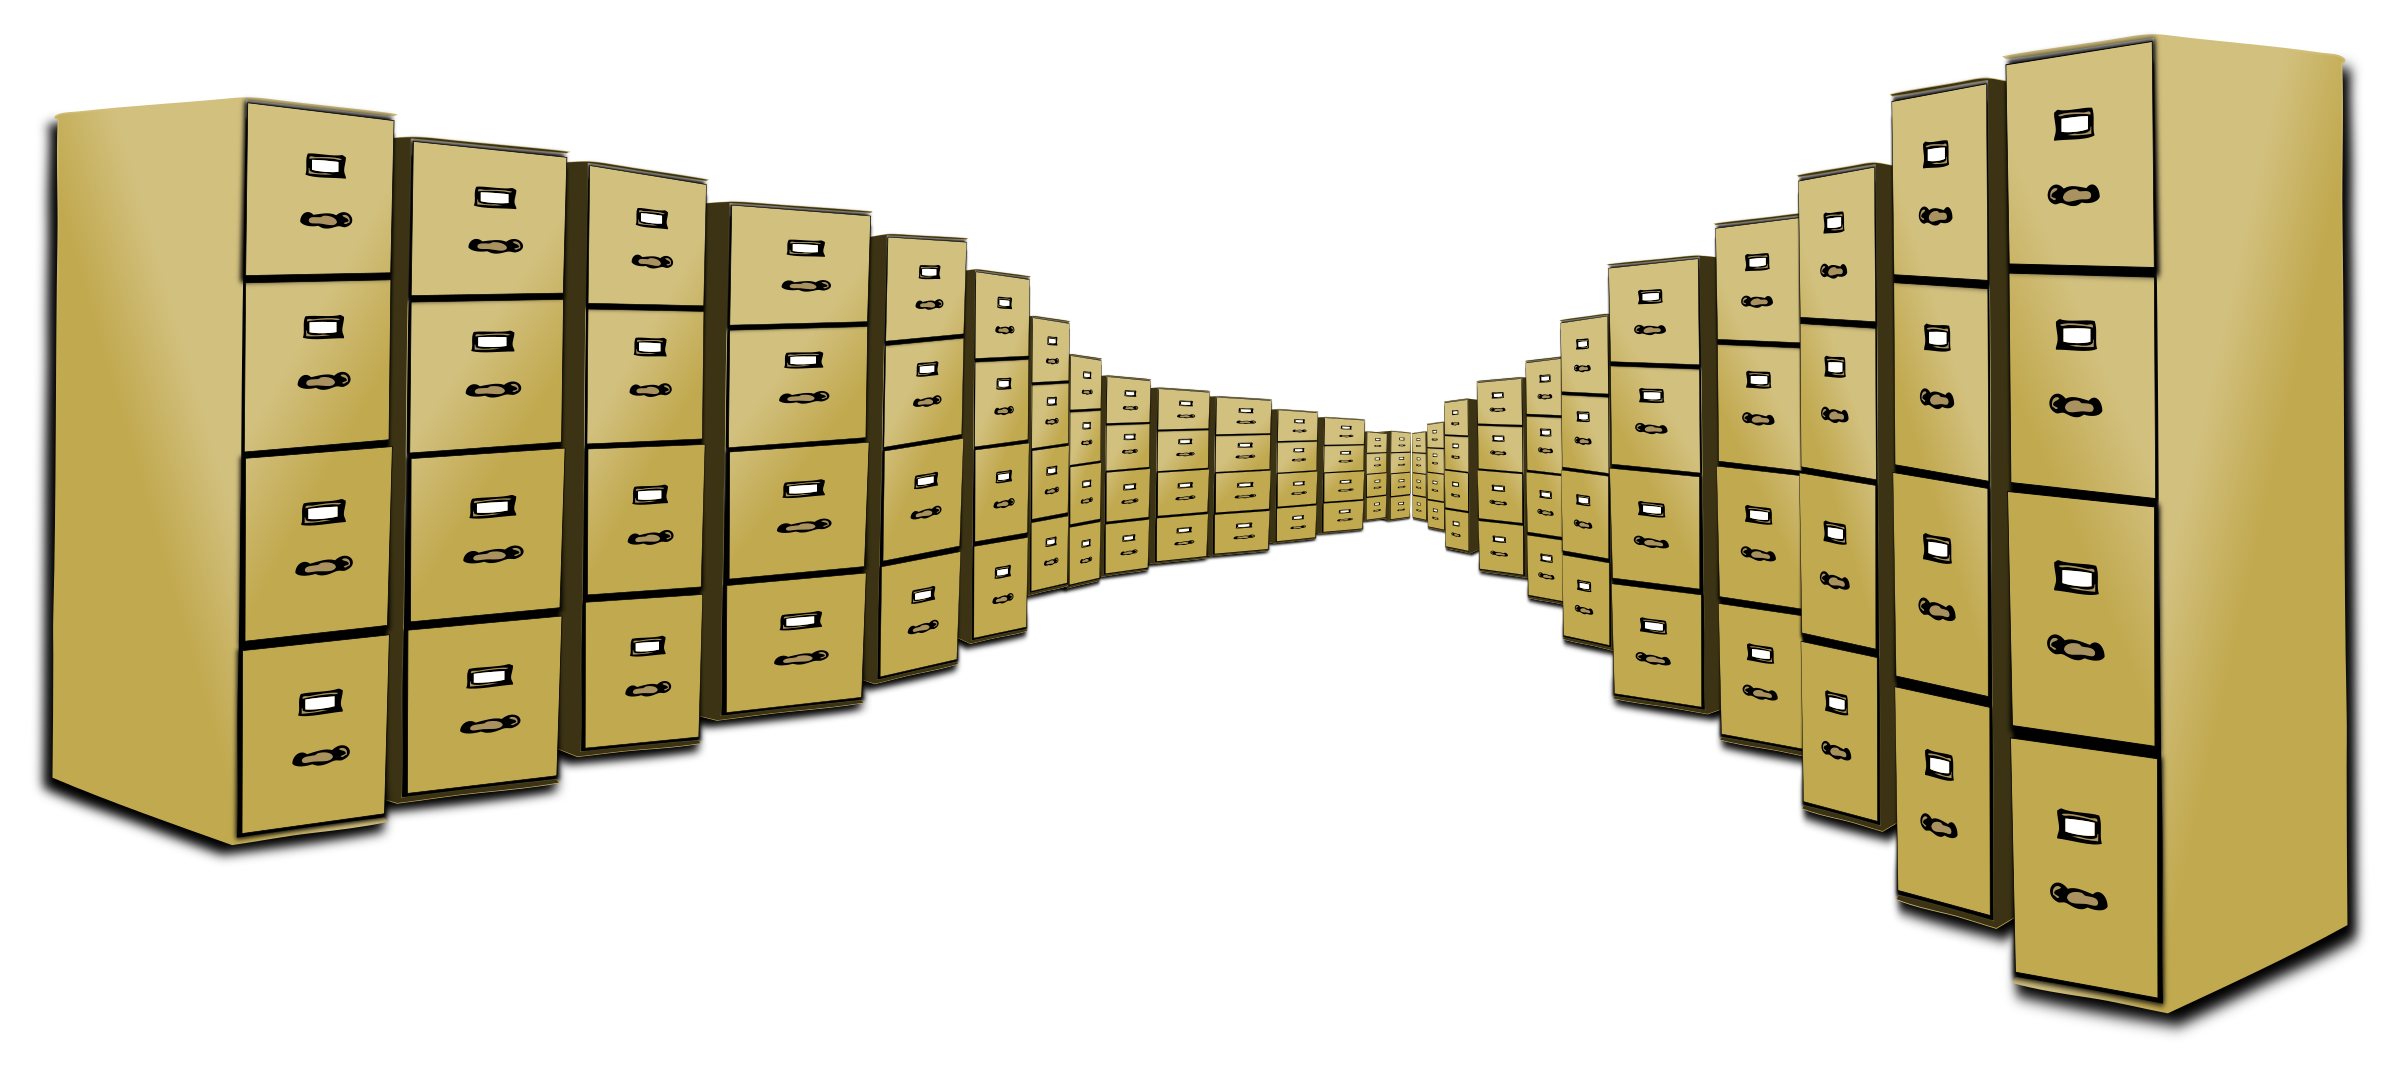
\includegraphics[scale=0.1]{storage.png} 
	\end{center}
	
	\begin{center}
	La blockchain est une technologie de \textbf{stockage} et de \textbf{transmission d’informations}, \textbf{transparente}, \textbf{sécurisée}, et fonctionnant \textbf{sans organe central de contrôle}.\footnote{\hspace{5pt}Définition de Blockchain France}
	\end{center}
	
	\begin{columns}
    	\begin{column}{0.48\textwidth}
    		\begin{center}
    			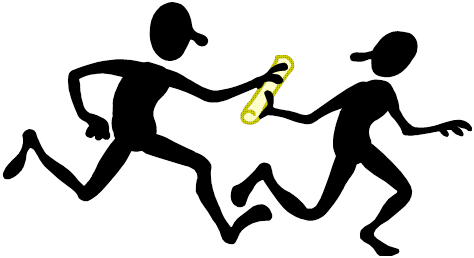
\includegraphics[scale=0.25]{relay.png} 
    		\end{center}
    	\end{column}
    	
    	\begin{column}{0.48\textwidth}
    		\begin{center}
				
\includegraphics[scale=0.25]{control.png} 
			\end{center}
    	\end{column}
	\end{columns}

% Liens  https://openclipart.org/detail/167738/filing-cabinet-overload
%		 http://worldartsme.com/relay-race-free-clipart.html#gal_post_57417_relay-race-free-clipart-1.jpg
%		 http://www.clipartpanda.com/clipart_images/security-bag-check-clip-art-58416511
\end{frame}

\begin{frame}{Introduction}{Objectifs}
	\vspace{-0.5cm}
	\begin{columns}
    	\begin{column}{0.48\textwidth}
    		\only<1-3>{
    		\begin{center}
    			\textbf{Durable\\}
    			\begin{figure}
    				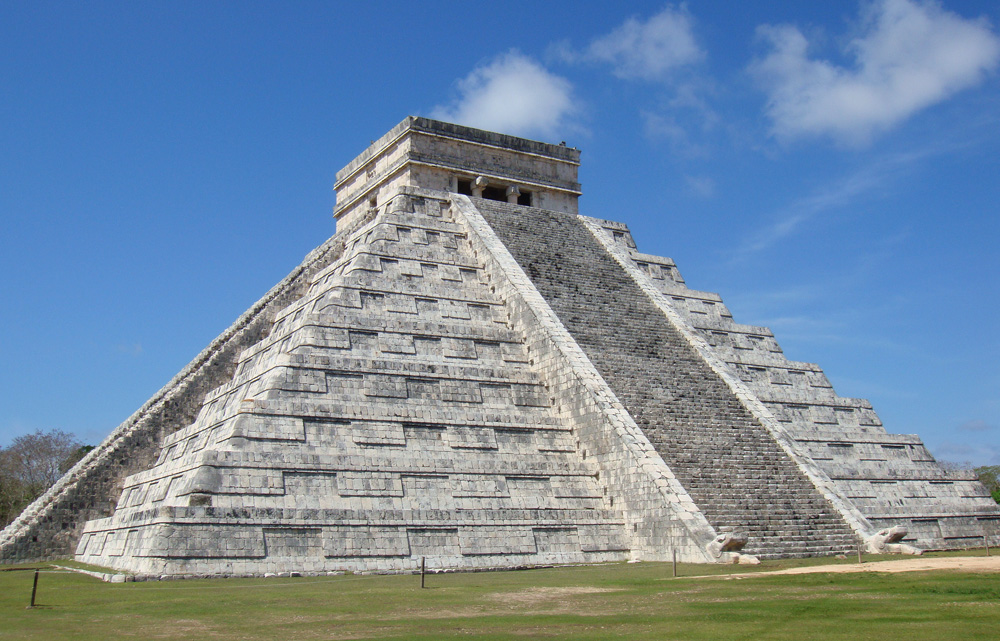
\includegraphics[scale=0.1]{perenity.jpg} 
    			\end{figure}
    		\end{center}}
    	\end{column}
    	
    	\begin{column}{0.48\textwidth}
			\only<2-3>{    		
    		\begin{center}
    			\textbf{Infalsifiable\\}
    			\begin{figure}
					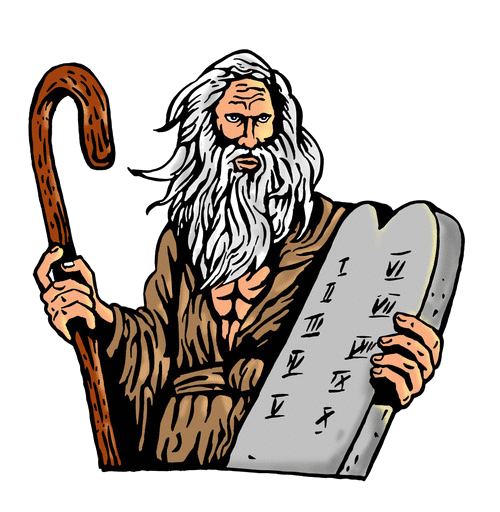
\includegraphics[scale=0.15]{commands.png} 
				\end{figure}
			\end{center}}
    	\end{column}
	\end{columns}
    		\only<3-3>{
    		\begin{center}
    			\textbf{Distribué\\}
    			\begin{figure}
    				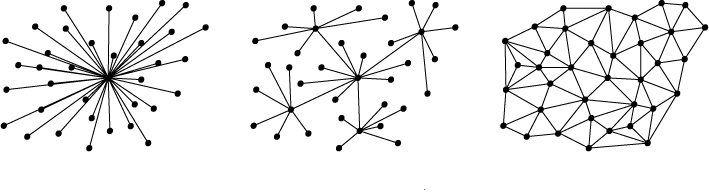
\includegraphics[scale=0.35]{central.png} 
    			\end{figure}
    		\end{center}}
% https://everestalexander.files.wordpress.com/2015/11/moses10commandmentstrans.gif
% http://zmeeed.info/aztec-architecture/popular-aztec-architecture-ancient-aztec-architecture-later-by-the-aztecs-th/
% http://blog.yintercept.com/2011/11/i-found-following-image-on-wikipedia.html
\end{frame}

\section{Fonctionnement}

\begin{frame}{Fonctionnement}{Hachage cryptographique}
	Exemple avec l'algorithme \textbf{SHA-256} :
	\vspace{1cm}
	\begin{center}
		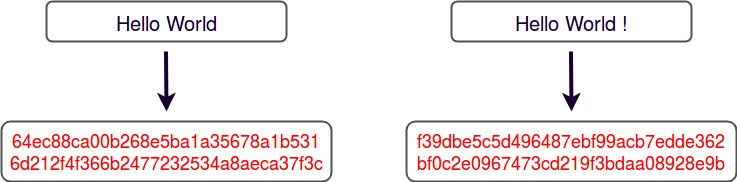
\includegraphics[scale=0.4]{hash.png} 
	\end{center}
\end{frame}

\begin{frame}{Fonctionnement}{Chaîne de blocs}
	\begin{center}
		\begin{figure}
			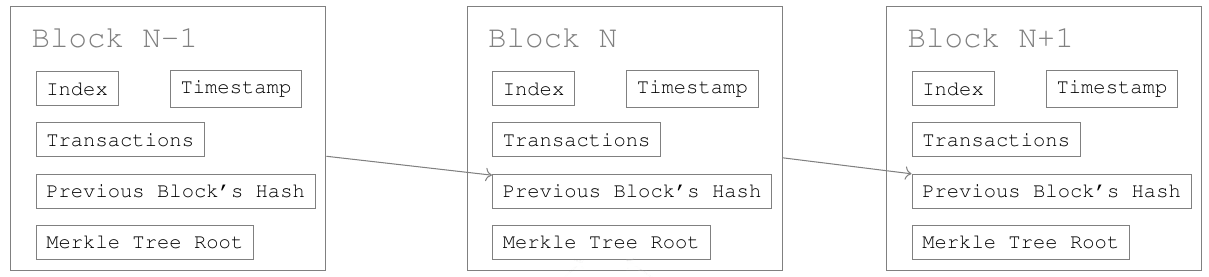
\includegraphics[scale=0.28]{blockk.png} 
		\end{figure}
	\end{center}
\end{frame}


\begin{frame}{Fonctionnement}{Merkle Tree}
	\only<1>{
	\begin{center}
		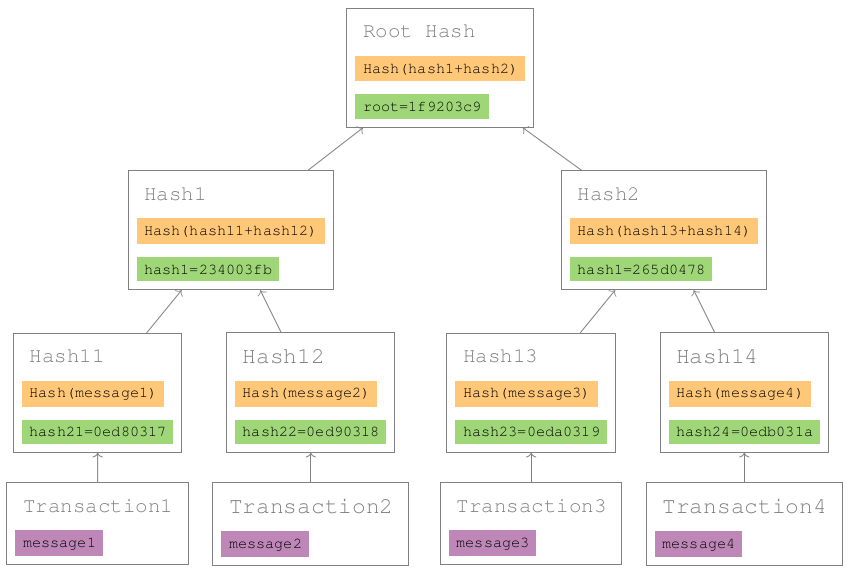
\includegraphics[scale=0.35]{merkle_tree_correct.png} 
	\end{center}}
	
	\only<2>{
	\begin{center}
		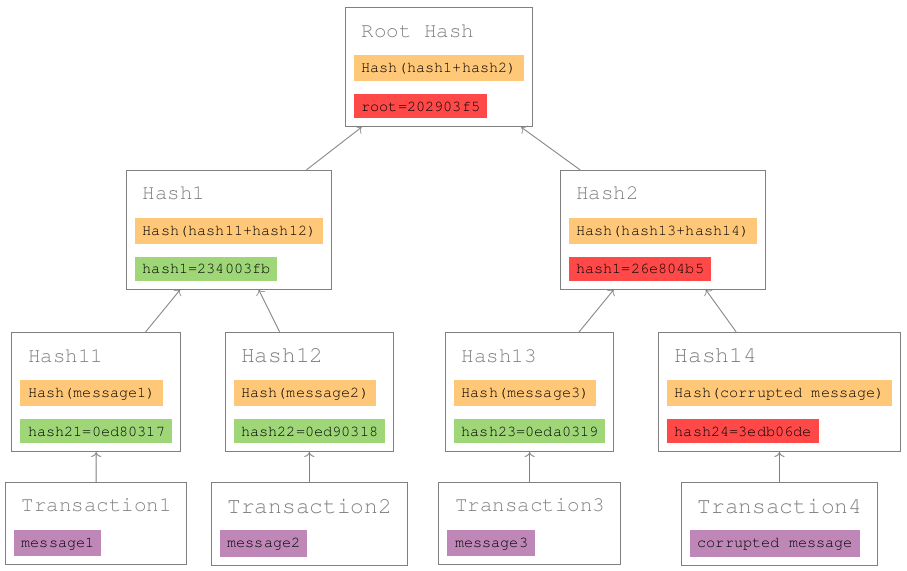
\includegraphics[scale=0.35]{merkle_tree_incorrect.png} 
	\end{center}}
\end{frame}


\begin{frame}{Fonctionnement}{Preuve de travail}
	\only<1-2>{
	\begin{center}
		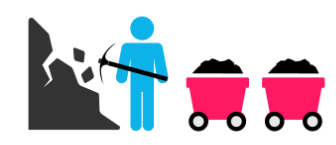
\includegraphics[scale=0.4]{mining.png}
	\end{center}
	\begin{center}
		La preuve de travail (\textbf{proof-of-work)} est un algorithme de consensus dans un réseau de Blockchain. Cet algorithme est utilisé pour confirmer les transactions et produire des nouveaux blocks dans la chaine en prouvant que des calculs informatiques onéreux ont été fait.
	\end{center}
	\begin{center}
		\begin{itemize}
			\item Utilisé par la plupart des crypto-monnaies (BTC,ETH,...)
			\item Les transactions du block ajouté sont valides (\textcolor{blue}{pourquoi ?})
		\end{itemize}
	\end{center}}
	\only<2-2>{
		\begin{center}
			\textbf{"Mentir a un coût financier!"}
		\end{center}}
\end{frame}

\begin{frame}{Fonctionnement}{Preuve de travail}
\begin{figure}
		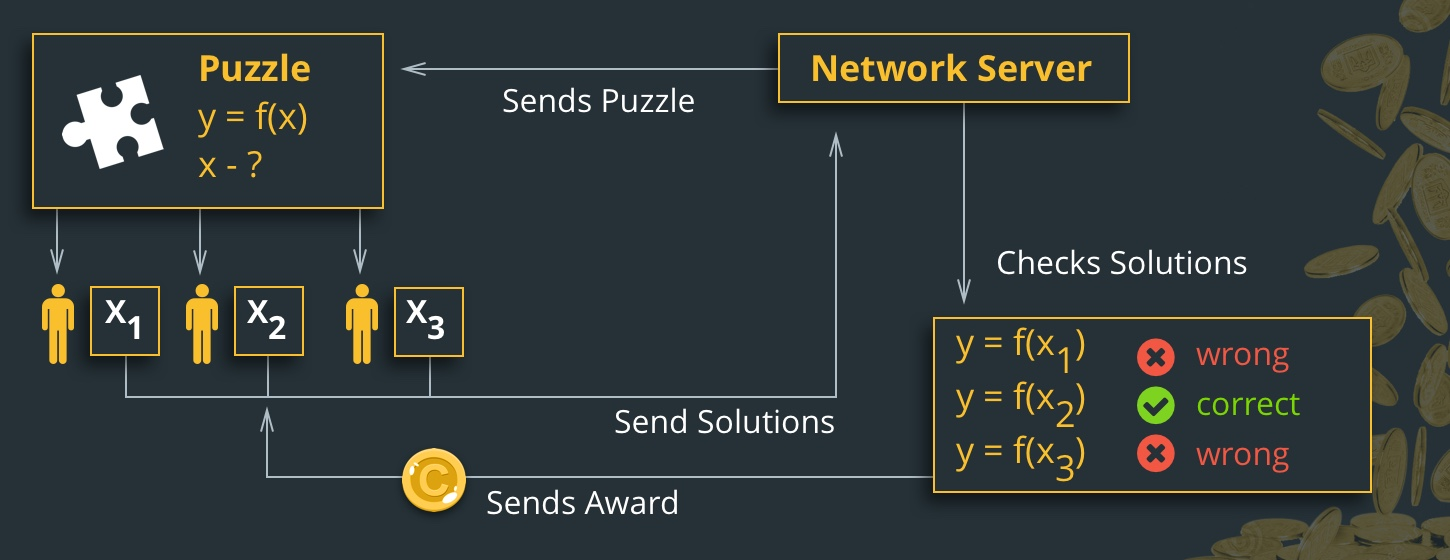
\includegraphics[scale=0.15]{pow.jpg} 
		\caption{proof-of-work(https://cointelegraph.com)}
	\end{figure}
	
	\begin{center}
		\begin{itemize}
			\item Le puzzle doit être compliqué à résoudre mais la solution est facile à vérifier
			\item Le puzzle ne doit être ni trop compliqué ni trop facile
			\item Le temps moyen pour ajouter un block est de 10 minutes
			\item Plus il y a de la puissance informatique ajoutée dans le réseau, plus compliqués seront les puzzle
		\end{itemize}
	\end{center}
\end{frame}

\section{Bitcoin}

\begin{frame}{Caractéristiques}
	\begin{center}
		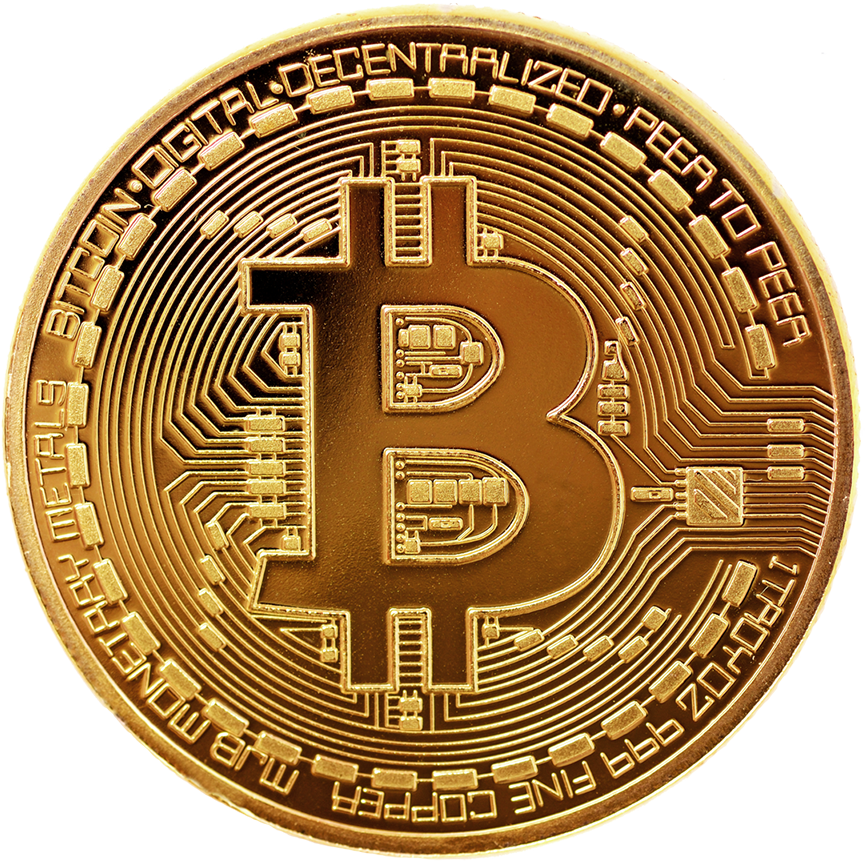
\includegraphics[scale=0.05]{bitcoinLogo.png}
	\end{center}
	
	\begin{center}
		\begin{itemize}
			\item Utilise la technologie Blockchain
			\item Limite de Bitcoins $\approx$ 21 millions (déjà 80\% minés)
			\item La récompense donnée à un mineur est d'environ 12.5 BTC 
			\item Comment stocker ses BTC ? Dans un "porte-feuille digital" (logiciel)
		\end{itemize}
	\end{center}
	\begin{center}
		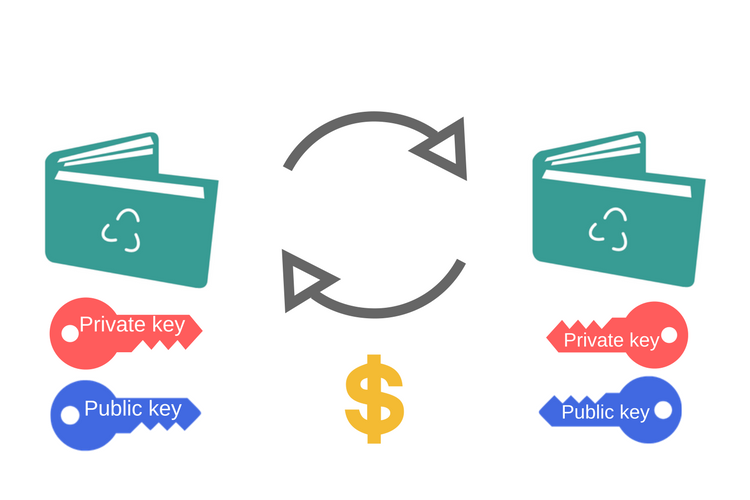
\includegraphics[scale=0.15]{wallets.png}
	\end{center}
\end{frame}

\section{Smart Contract}

\begin{frame}{Smart Contract}
	
	
	\begin{center}
		Nick Szabo, \textit{Smart Contracts: Building Blocks for Digital Markets}, 1996
	\end{center}		
	
	\begin{figure}
		\centering
		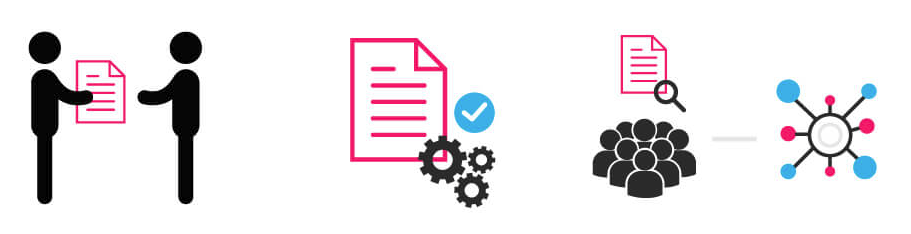
\includegraphics[scale=.25]{smart_contract}
		\caption{[Public domain]}
	\end{figure}
	
	
\end{frame}

\begin{frame}{Smart Contract}{Exemple d'Assurance}

	\begin{figure}
		\centering
		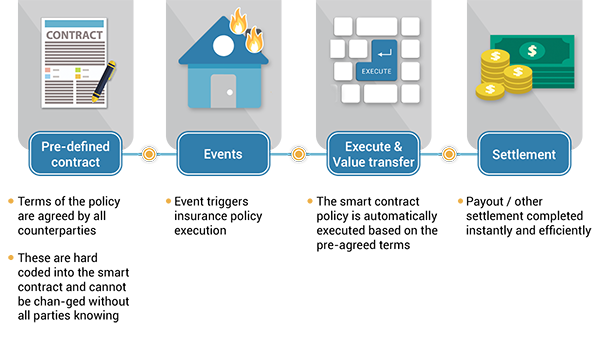
\includegraphics[scale=.48]{insurance_contract}
		\caption{Par draglet GmbH [CC BY-SA 4.0 (https://creativecommons.org/licenses/by-sa/4.0)], de Wikimedia Commons}
	\end{figure}

\end{frame}

\begin{frame}{Smart Contract}{Exemple de code de contrat}

	\begin{figure}
		\centering
		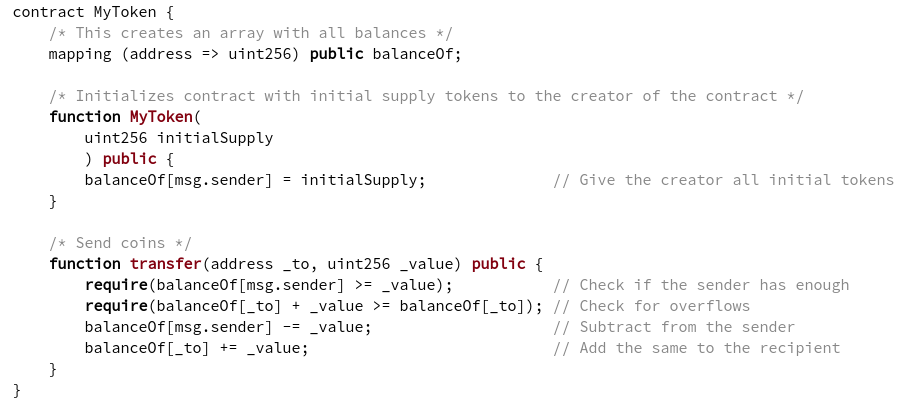
\includegraphics[scale=.35]{contract_example}
		\caption{Exemple de smart contract sur Ethereum. https://www.ethereum.org/token}
	\end{figure}

\end{frame}

\begin{frame}{Smart Contract}{Ethereum Tokens}

	\begin{center}
		\color{blue}
		Smart Contract de Ethereum permet de créer des blockchains sur la base de leur blockchain
	\end{center}
	
	Exemple:
	\begin{figure}
	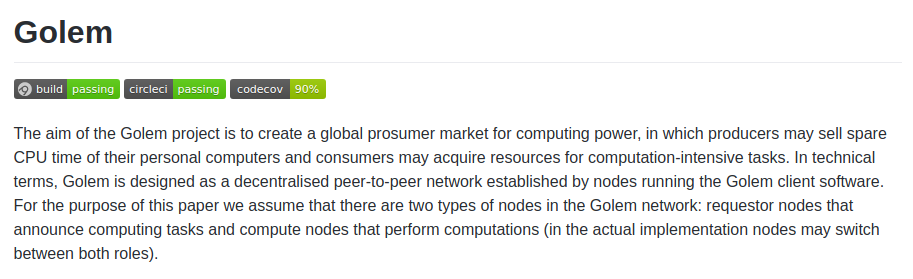
\includegraphics[scale=.35]{golem}
	\caption{Source: Github de Golem}
	\end{figure}

\end{frame}

\section{Conclusion}

\begin{frame}{Conclusion}{Quelques implementations intéressantes de Blockchain}

	\begin{itemize}
		\item L'Estonie a complètement digitalisé les données de ses citoyens.
		\item Régulation du commerce des poissons grâce à Hyperledger Sawtooth.
		\item Test de smart cities à Dubai.
		\item Votes électroniques à Moscou en 2014.
	\end{itemize}
	
\end{frame}

\end{document}
